\documentclass[12pt]{article}
\usepackage[margin=1in]{geometry}
\usepackage{amsmath,amssymb,amsthm,booktabs,graphicx,natbib,microtype,array}
\newtheorem{theorem}{Theorem}
\newtheorem{corollary}[theorem]{Corollary}
\newtheorem{proposition}[theorem]{Proposition}
\newtheorem{remark}[theorem]{Remark}
\title{Conditional Source-to-Directional-Support Composition\\\large Quantitative Interface Gates from Snapshot Balls to Support Cocycles}
\author{Prime Dynamics Theory Program}
\date{July 2026}

\begin{document}
\maketitle

\begin{abstract}
We assemble the enclosure and viability layers into one conditional theorem.
At level $n$, assume: an exact normalized source snapshot lies in an operator
ball of radius $\varepsilon_n$ around a computed snapshot; the computed
packet has approximate spectral gap $g_n>2\varepsilon_n$; the induced packet
and source radii propagate below the strict threshold-branch margin; the
resulting exact branch admits outward-validated tail and normalized-base
transitions
\[
 x_n\leq y_n,
 \qquad y_{n+1}\leq F_{n,c_n}(y_n),
 \qquad a_{n+1}\geq r_{n,c_n}a_n;
\]
and, after a validated reset, the correlated multipliers
\[
 \kappa_n=r_{n,c_n}
 \frac{(1-\sqrt{F_{n,c_n}(y_n)})_+^4}{(1-\sqrt{y_n})^4}
\]
have partial logarithmic sums bounded below by $-C$.  Then the actual
directional candidate satisfies
\[
 a_n(1-\sqrt{x_n})_+^4\geq
 a_N(1-\sqrt{y_N})^4e^{-C}>0
\]
for every later level.  Four omission witnesses show that the gap, branch,
outward-dominance, and cocycle packets cannot simply be deleted from this
proof architecture.

An automated readiness audit verifies all eight RH-140--RH-147 archives and
the RH-138 outward reference.  The finite checkpoints are strong but not yet
one end-to-end interval proof: 10/10 factorized source packets, 360/360 strict
nominal branch margins, 330/330 outward residual pairs, 28/30 positive support
tubes, and an 18/18 delayed clean suffix.  Three all-level interfaces remain:
uniform source/packet enclosure, propagation of packet balls through the
thresholded recursion into the outward assembly, and a delayed support
cocycle with uniformly bounded drawdown.  Hence the theorem is a rigorous
composition rule, not a claim that directional Stage A is closed.
\end{abstract}

\section{The interface problem}
The preceding papers establish exact local theorems, but a proof is only as
strong as the interfaces between them.  A spectral packet certified from one
source approximation cannot be inserted silently into a later recurrence
computed from unvalidated floating-point matrices.  Likewise, a finite
positive directional floor cannot be promoted to an all-level liminf without
a reset and a recurrent support estimate.

We therefore state the entire source-to-support route in one theorem.  Its
purpose is twofold: to make every quantitative handoff explicit and to
separate a complete logical implication from the still-missing hypotheses.
The perturbation ingredients are standard operator and interval methods
\citep{Kato1995,Bhatia2007,Moore1966}; the final controlled step uses the
viability language developed in RH-144--RH-147 \citep{Aubin1991}.

Let $S_n$ be the exact normalized source snapshot and $\widehat S_n$ its
computed center.  Let $P_n$ and $\widehat P_n$ be the exact and computed
rank-four packet projectors.  The recursive packet update contains a clipped
relative singular-value threshold, so its selected width is locally constant
only inside a strict branch radius.

\section{Quantitative gates}
The first gate is the approximate spectral gap.  Suppose
\begin{equation}\label{eq:source}
 \|S_n-\widehat S_n\|\leq\varepsilon_n
\end{equation}
and the computed cluster-to-complement gap is $g_n>2\varepsilon_n$.  The
RH-141 projector estimate gives
\begin{equation}\label{eq:packet}
 \|P_n-\widehat P_n\|leq
 p_n:=\frac{\varepsilon_n}{g_n-\varepsilon_n}.
\end{equation}
The strict factor two ensures the target cluster remains isolated on both
sides of the perturbation.

Let $m_n>0$ be the exact threshold-branch radius from RH-143 and let
\begin{equation}\label{eq:branch}
 q_n=L_n^{(S)}\varepsilon_n+L_n^{(P)}p_n+\rho_n^{\rm round}
\end{equation}
be an outward propagated cross-matrix radius.  The branch gate is
$q_n<m_n$.  Under this strict inequality, the exact and computed updates
select the same width and clipping branch.  Equality is deliberately
excluded because it permits contact with the threshold surface.

On that branch, assume an outward residual calculation produces a monotone
tail map $F_{n,c}$ and a positive base-ratio lower $r_{n,c}$ satisfying, for
the actual matrices,
\begin{equation}\label{eq:outward}
 x_n\leq y_n,
 \qquad
 y_{n+1}\leq F_{n,c_n}(y_n),
 \qquad
 a_{n+1}\geq r_{n,c_n}a_n.
\end{equation}
This hypothesis includes the source-to-assembly radii and both RH-138 Loewner
residual guards; a nominal recurrence is not enough.

\section{Conditional composition theorem}
Write $\phi(y)=(1-\sqrt y)_+^4$ and define the actual directional candidate
\[
 B_n=a_n\phi(x_n).
\]

\begin{theorem}[Source-to-directional-support composition]\label{thm:composition}
Suppose that after some level $N$:
\begin{enumerate}
\item the source and packet gates \eqref{eq:source}--\eqref{eq:packet} hold;
\item the strict branch gate $q_n<m_n$ holds at every update;
\item the outward transition \eqref{eq:outward} holds for selected controls
$c_n$ and $F_{n,c_n}(y_n)<1$;
\item a validated reset gives $a_N\phi(y_N)>0$; and
\item for some finite $C$ and every $n>N$,
\begin{equation}\label{eq:cocycle}
 \sum_{j=N}^{n-1}\log\!\left(
 r_{j,c_j}\frac{\phi(F_{j,c_j}(y_j))}{\phi(y_j)}
 \right)\geq-C.
\end{equation}
\end{enumerate}
Then for every $n\geq N$,
\begin{equation}\label{eq:conclusion}
 B_n\geq a_N\phi(y_N)e^{-C}>0.
\end{equation}
In particular the actual directional candidates have a positive eventual
liminf.
\end{theorem}

\begin{proof}
The source gap and branch gates ensure that the outward transition applies to
the actual recursively selected packet, rather than only to a nominal branch.
Because $x_n\leq y_n$ and $\phi$ is decreasing,
$B_n\geq a_n\phi(y_n)$.  RH-147's sharp correlated multiplier and
\eqref{eq:outward} give
\[
 a_{n+1}\phi(y_{n+1})\geq
 r_{n,c_n}\frac{\phi(F_{n,c_n}(y_n))}{\phi(y_n)}
 a_n\phi(y_n).
\]
Iterating and applying \eqref{eq:cocycle} proves \eqref{eq:conclusion}.
\end{proof}

The theorem accommodates RH-145 delayed start: no hypothesis is needed on a
finite prefix before $N$.  It also allows local support losses, provided the
signed cocycle drawdown remains bounded.

\section{Four omission witnesses}
Each interface carries genuine information.

\begin{proposition}[Architecture-relative necessity]\label{prop:witnesses}
None of the gap, strict branch, outward-dominance, or cocycle packets can be
removed from Theorem~\ref{thm:composition} while retaining its conclusion
from the remaining scalar data alone.
\end{proposition}
\begin{proof}
For the gap packet, a two-dimensional matrix with a double eigenvalue has no
distinguished rank-one packet; arbitrarily small perturbations can rotate the
chosen eigenspace.  At $g=2\varepsilon$ the quantitative denominator reaches
the separation wall.

For the branch packet, place a singular value exactly at the clipped relative
threshold.  Perturbations of either sign select different widths, so equality
$q=m$ is insufficient.

For outward dominance, let the nominal tail be zero but the actual tail
equal one.  The nominal support is positive while the actual support
vanishes; no nominal calculation repairs the missing enclosure.

For the cocycle packet, take every multiplier equal to $1/2$.  All local
quantities are positive, yet the equality support trajectory is $2^{-n}$ and
has zero liminf.
\end{proof}

These witnesses are relative to this modular proof system.  A different
argument may replace a packet with stronger structural information, but it
cannot simply omit the issue the packet controls.

\section{Finite readiness audit}
Table~\ref{tab:readiness} records the strongest finite checkpoint and the
corresponding open all-level interface.  All eight archive-verification files
and summary hashes pass; none asserts Stage A or the Riemann Hypothesis.

\begin{table}[t]
\centering
\scriptsize
\renewcommand{\arraystretch}{1.12}
\begin{tabular}{cclp{5.0cm}}
\toprule
RH & layer & finite checkpoint & missing all-level packet\\
\midrule
140 & source ball & 10/10 rank-four radii below $10^{-3}$ & uniform normalized-source enclosure\\
141 & packet gap & 4/10 universal; 10/10 quadratic diagnostic & interval-valid quadratic packet radius\\
142 & Arb packet & 10/10 frozen binary packets & uniform packet theorem\\
143 & branch gate & 360/360 strict nominal margins & propagate packet balls through recursion\\
144 & control kernel & 28/30 viable chains & all-level repeating/reset block\\
145 & delayed start & 18/18 clean suffix & exclude recurrent future bad births\\
146 & base recurrence & 330/330 bounds, direct product lossy & positive all-level base/cancellation packet\\
147 & support tube & 28/30 common positive tubes & all-level lower-bounded support cocycle\\
\bottomrule
\end{tabular}
\caption{Readiness of the RH-140--RH-147 interface stack.}
\label{tab:readiness}
\end{table}

The RH-138 reference contributes 330/330 successful raw and bridge residual
pairs, but its own claim boundary says that the reference assembly is not an
interval source model.  Thus the finite numbers cannot be multiplied into an
end-to-end theorem.  In particular, RH-142 packet balls have not yet been
propagated through all RH-143 threshold updates into the exact Gram and tail
matrices used by RH-138.

An independent 4,096-instance synthetic audit exercises the quantitative
gap, branch, outward, and cocycle gates.  Every actual synthetic support
trajectory dominates the theorem floor.  All four omission witnesses are
also machine checked.

\begin{figure}[t]
\centering
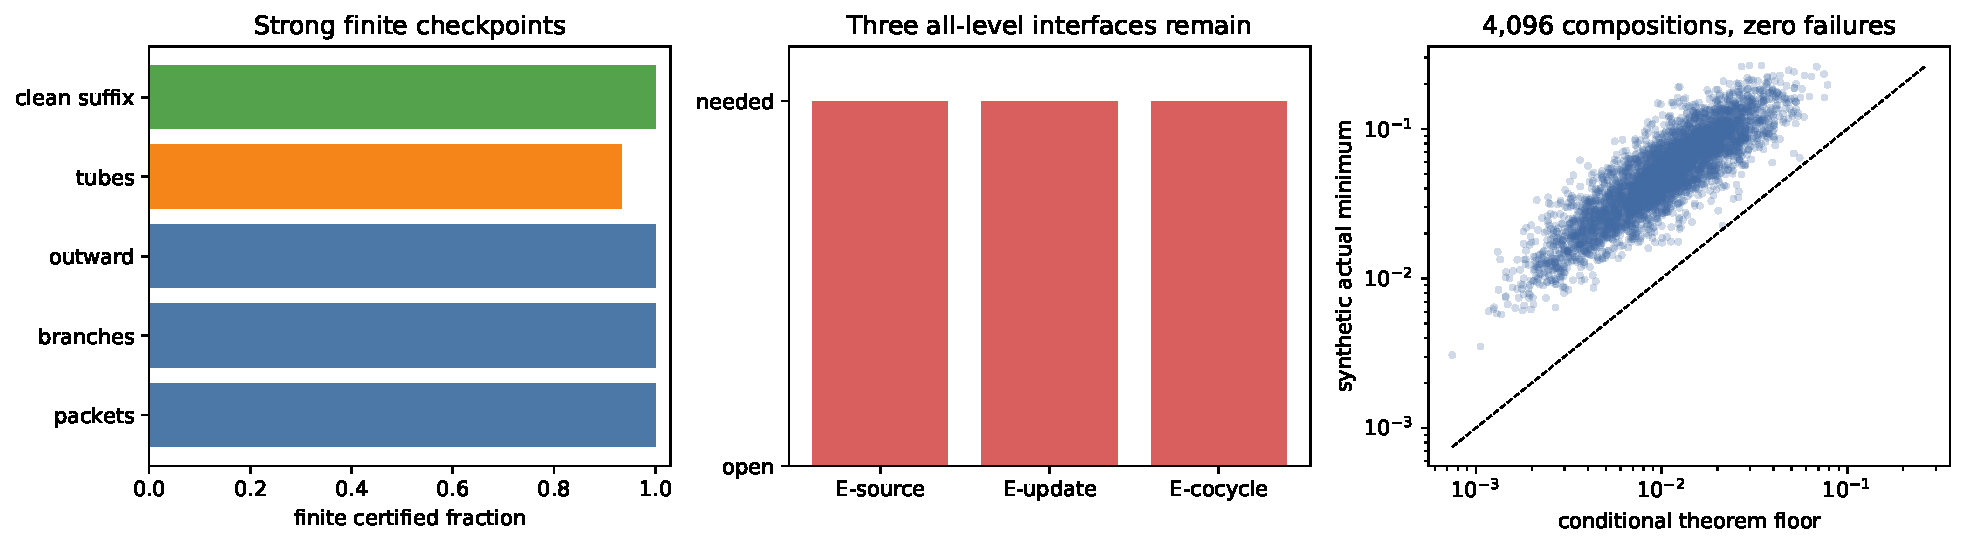
\includegraphics[width=\textwidth]{figures/source_directional_support_composition.pdf}
\caption{Strong finite checkpoints, the three open all-level interfaces, and
the synthetic conditional-composition audit.}
\label{fig:composition}
\end{figure}

\section{The reduced frontier and claim boundary}
The proof architecture now has three open interfaces rather than a diffuse
list of numerical observations:
\[
 \boxed{E_{\rm source}:\ \text{all-level source and packet balls}},
\]
\[
 \boxed{E_{\rm update}:\ \text{branch-stable propagation into the outward assembly}},
\]
\[
 \boxed{E_{\rm cocycle}:\ \text{delayed support cocycle with bounded drawdown}}.
\]
Once all three are proved on one common construction, Theorem
\ref{thm:composition} supplies eventual positive directional support without
another conceptual step.  The interfaces may be attacked separately, but
their enclosures must be compatible.

RH-148 proves the conditional implication and audits finite readiness.  It
does not close a finite end-to-end interval source-to-support path, prove any
of the three all-level interfaces, establish uniform Stage A, construct a
Hilbert--Polya operator, identify zeta zeros, or prove the Riemann Hypothesis.

\bibliographystyle{plainnat}
\bibliography{references}
\end{document}

